\section{ЕКОНОМІЧНА ДОЦІЛЬНІСТЬ ВИКОРИСТАННЯ ПРОГРАМНОГО ЗАБЕЗПЕЧЕННЯ}

\subsection{Економічна доцільність розробки програмного забезпечення та його впровадження}

В даному проекті необхідно реалізувати корпоративну систему для спільної і одночасної роботи працівників деякої компанії. В ньому буде реалізовано систему обміну повідомленнями, управління задачами і завданнями, зручне ведення корпоративного календаря, спільна робота над документами різного типу (текстові документи, презентації тощо), система корпоративної вікі та блог. 
\par Як відомо, кожний продукт, який розробляється сьогодні з подальшим впровадженням на ринок потребує обґрунтування з економічної точки зору, а саме доцільності даного продукту. Дане обґрунтування необхідне для того, щоб вчасно припинити (при втраті актуальності або надмірних витратах) розробку або здійснити необхідні інвестування в проект для забезпечення необхідними програмними або апаратними засобами розробників з метою одержання очікуваних результатів. Економічний ефект розробленого продукту визначається на основі економічних показників, які дають можливість прогнозувати результат від впровадження даного програмного продукту.
\par Існує багато методів визначення економічних показників доцільності впровадження та використання будь якого програмного продукту. Враховуючи інтенсивне впровадження комп’ютерної техніки в корпоративній сфері, на сьогодні такий аналіз є невід’ємною частиною попереднього аналізу аналогічних робіт, оскільки саме результат економічних показників доцільності дозволяє визначити доцільність розробки програмного продукту.
\par В даній роботі проводиться розрахунок економічних показників та аналіз всієї роботи по розробці корпоративної системи.

\subsection{Побудова мережевого графа}
Мережевий граф є основним плановим документом в системі мережевого планування і керування, що являє собою інформаційно-динамічну модель, в якій зображуються взаємозв'язки і результати всіх робіт, необхідних для досягнення кінцевої мети розробки, тобто мережевий граф - це наочне відображення плану робіт.
\par В мережевому графі детально чи укрупнено показано, що, в якій послідовності, коли, за який час, для чого необхідно виконати, щоб забезпечити закінчення всіх робіт не пізніше заданого, директивного терміну.
\par Порядок побудови мережевих графів визначається прийнятою технологією і організацією робіт. Мережеві графи тільки відображають існуючу або проектовану черговість і взаємозв'язок виконання робіт.
\par По кожній роботі необхідно враховувати:
\begin{itemize}
	\item які роботи повинні бути завершені раніше, ніж почнеться дана робота;
	\item які роботи можуть початись після завершення даної роботи;
	\item які інші роботи повинні виконуватись одночасно з виконуванням даної роботи.
\end{itemize}
\par Аналізуючи мережевий граф можна виділити його головні елементи: події і роботи. Розглянемо детальніше значення термінів:
\begin{itemize}
	\item подія - це стан, момент досягнення проміжної або кінцевої цілі розробки.
	\item робота - це розтягнений в часі процес, необхідний для здійснення події. Кожна робота має попередню подію і закінчується визначеною подією.
\end{itemize}

\par На мережевих графах подія відображається колом, а робота -- стрілкою. До основних параметрів мережевого графа відносяться: критичний шлях, резерви часу подій. Ці параметри є вихідними для одержання ряду додаткових характеристик, а також для аналізу мережі чи для аналізу складеного плану розробки.
\par Резерв часу події - це такий проміжок часу, на який може бути відкладене здійснення цієї події без порушення термінів завершення розробки в цілому. Резерви часу існують в мережевому графі в усіх випадках, коли існує більш ніж один шлях різної тривалості.
\par Резерв часу події К визначається як різниця між пізнім $T_{p}$ і раннім $T_{r}$ термінами завершення події за формулою

\begin{equation}
	K=\frac{T_{p}}{T_{r}}
\end{equation}

\par Найбільш пізній з допустимих термінів $T_{p}$ -- це такий термін здійснення події, перевищення якого викличе аналогічну затримку завершальної події. Іншими словами, якщо подія наступила в момент $T_{p}$, вона потрапила в критичну зону і наступні за нею роботи повинні знаходитись під таким же контролем як і роботи критичного шляху.

\par Найбільш ранній з можливих термінів здійснення події $T_{p}$ -- це термін необхідний для виконання всіх робіт, що передують цій події. Цей час знаходиться шляхом вибору максимального значення із тривалості всіх шляхів, що приводять до даної події.
\par Вихідні дані мережевого графа представлені в таблицях \ref{t:eco_1} та \ref{t:eco_2}.


{\footnotesize
\begin{longtable}{|c|c|}

\captionsetup{justification=centering}
\caption{Події мережевого графа}\label{t:eco_1}\\
\hline
\multicolumn{1}{|c|}{\textbf{№ події}}&
\multicolumn{1}{c|}{\textbf{Подія}}\\\hline

\endfirsthead
\caption*{\hfill Продовження таблиці \ref{t:eco_1}}\\\hline

\multicolumn{1}{|c|}{\textbf{№ події}}&
\multicolumn{1}{c|}{\textbf{Подія}}\\\hline
\endhead

0 & Отримання завдання на дипломне проектування\\ \hline
1 & Аналіз проблеми дипломного проектування \\ \hline
2 & Ознайомлення з літературою на задану тему \\ \hline
3 & Пошук інформації в мережі INTERNET \\ \hline
4 & Підбір необхідних джерел інформації  \\ \hline
5 & Аналіз підібраного матеріалу  \\ \hline
6 & Визначення задач, які виникають при розробці  \\ \hline
7 & Розгляд існуючих способів розробки корпоративних систем \\ \hline
8 & Аналіз існуючих способів розробки  \\ \hline
9 & Пошук існуючих корпоративних систем \\ \hline
10 & Аналіз знайдених аналогів та їх функціональності \\ \hline
11 & Розробка структури алгоритму  \\ \hline
12 & Розробка алгоритму програми  \\ \hline
13 & Вибір серверної  платформи для реалізації завдання  \\ \hline
14 & Визначення основних та допоміжних програмних модулів  \\ \hline
15 & Реалізація програмних модулів в середовищі програмування  \\ \hline
16 & Попереднє налагодження програмних модулів \\ \hline
17 & Остаточне налагодження програми \\ \hline
18 & Тестування програмного продукту \\ \hline
19 & Визначення економічної доцільності використання програми \\ \hline
20 & Завершення роботи АБВГ\\ \hline

\end{longtable}
}


{\footnotesize
\begin{longtable}{|c|c|c|}
\captionsetup{justification=centering}
\caption{Роботи мережевого графа}\label{t:eco_2}\\
\hline
\multicolumn{1}{|c|}{\textbf{Номери робіт}}&
\multicolumn{1}{c|}{\textbf{Роботи}}&
\multicolumn{1}{c|}{\textbf{Тривалість, \newline дні}}\\\hline

\endfirsthead
\caption*{\hfill Продовження таблиці \ref{t:eco_2}}\\\hline

\multicolumn{1}{|c|}{\textbf{Номери робіт}}&
\multicolumn{1}{c|}{\textbf{Роботи}}&
\multicolumn{1}{c|}{\textbf{Тривалість, дні}}\\\hline
\endhead

0-1 & Аналіз завдання дипломного проекту & 2\\ \hline
1-2 & Огляд літератури & 3\\ \hline
1-3 & Огляд інформації в INTERNET & 3\\ \hline
3-4 & Робота з підібраним матеріалом з INTERNET & 4\\ \hline
2-4 & Робота з підібраним технічним матеріалом & 3\\ \hline
4-5 & Аналіз вимог до системи та її функціональності & 4\\ \hline
5-6 & Виділення та групування задач розробки & 3\\ \hline
6-7 & Пошук та розгляд існуючих методів реалізації & 7\\ \hline
7-8 & Аналіз та компонування існуючих способів розробки & 4\\ \hline
8-9 & Пошук аналогів розробленої системи & 5\\ \hline
8-10 & Аналіз аналогів розробленої системи & 4\\ \hline
9-11 & Завершення аналізу аналогів та вибір способу реалізації & 2\\ \hline
11-13 & Розробка структури алгоритму & 5\\ \hline
10-12 & Складання алгоритму програми та його аналіз & 2\\ \hline
12-13 & Розробка структури програми & 7\\ \hline
13-14 & Уточнення виду вхідних даних для програми & 5\\ \hline
14-15 & Аналіз інструментальних засобів створення програми & 2\\ \hline
15-16 & Підбір середовища програмування & 3\\ \hline
16-17 & Написання коду модулів програми & 14\\ \hline
17-18 & Налагодження всіх модулів програми & 7\\ \hline
18-19 & Завершення етапу налагодження програми & 3\\ \hline
19-20 & Тест програми та аналіз результатів тестування & 2\\ \hline
20-21 & Аналіз економічних показників & 5\\ \hline
21-22 & Завершення роботи & 14\\ \hline

\end{longtable}
}


\begin{center}
		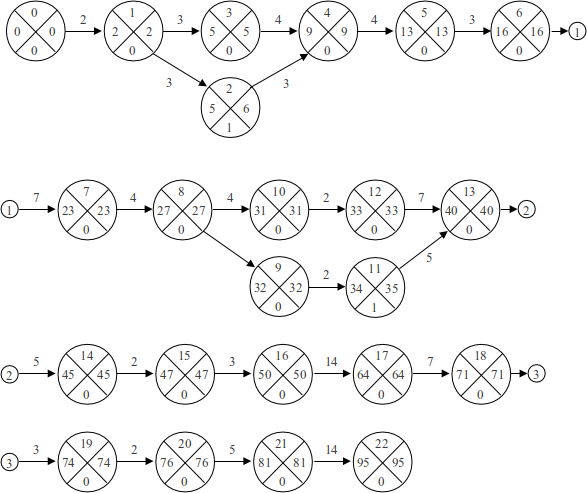
\includegraphics[width=1.00\textwidth]{ecomonic_graph.png}
		\captionof{figure}{Мережевий граф виконаних робіт}\label{t:eco_graph}
\end{center}

\par На рисунку \ref{t:eco_graph} зображений мережевий граф, який отримано із вихідних даних таблиць. Знаходимо критичний шлях і розраховуємо ранній, пізній час і резерв часу.
\par Критичний шлях --- це найбільш тривала по часу послідовність робіт, які ведуть від вихідної до завершальної події. Величина критичного шляху визначає термін виконання всього комплексу по плануванню робіт.
\par Зміна тривалості будь-якої роботи, що лежить на критичному шляху, відповідним чином змінює термін настання завершальної події, тобто дату досягнення кінцевої мети, яка ставиться при плануванні розробки.
\par При плануванні комплексу операцій критичний шлях дозволяє знайти термін настання завершальної події. В процесі керування ходом розробки увага керівництва зосереджується на роботах критичного шляху. Це дозволяє найбільш  доцільно   і   оперативно  контролювати   обмежене  число  робіт, що впливають на термін розробки, а також краще використати існуючі ресурси.
\par Оскільки в даному випадку мережевий граф досить простий, очевидно що критичний шлях рівний 95.
\par Дані розрахунків часу подій приведені в таблиці \ref{t:eco_3}.


{\footnotesize
\begin{longtable}{|c|c|c|c|}

\captionsetup{justification=centering}
\caption{Параметри подій мережевого графіка}\label{t:eco_3}\\
\hline
\multicolumn{1}{|c|}{\textbf{№ події}}&
\multicolumn{1}{c|}{\textbf{Ранній час}}&
\multicolumn{1}{c|}{\textbf{Пізній час}}&
\multicolumn{1}{c|}{\textbf{Резерв часу}}\\\hline

\endfirsthead
\caption*{\hfill Продовження таблиці \ref{t:eco_3}}\\\hline

\multicolumn{1}{|c|}{\textbf{№ події}}&
\multicolumn{1}{c|}{\textbf{Ранній час}}&
\multicolumn{1}{c|}{\textbf{Пізній час}}&
\multicolumn{1}{c|}{\textbf{Резерв часу}}\\\hline
\endhead

0 & 0 & 0 & 0\\ \hline
1 & 2 & 2 & 0\\ \hline
2 & 5 & 6 & 1\\ \hline
3 & 5 & 5 & 0\\ \hline
4 & 9 & 9 & 0\\ \hline
5 & 13 & 13 & 0\\ \hline
6 & 16 & 16 & 0\\ \hline
7 & 23 & 23 & 0\\ \hline
8 & 27 & 27 & 0\\ \hline
9 & 32 & 32 & 0\\ \hline
10 & 31 & 31 & 0\\ \hline
11 & 34 & 35 & 1\\ \hline
12 & 33 & 33 & 0\\ \hline
13 & 40 & 40 & 0\\ \hline
14 & 45 & 45 & 0\\ \hline
15 & 47 & 47 & 0\\ \hline
16 & 50 & 50 & 0\\ \hline
17 & 64 & 64 & 0\\ \hline
18 & 71 & 71 & 0\\ \hline
19 & 74 & 74 & 0\\ \hline
20 & 76 & 76 & 0\\ \hline
21 & 81 & 81 & 0\\ \hline
22 & 95 & 95 & 0\\ \hline

\end{longtable}}

\subsection{Економічне обґрунтування розробки та впровадження програми}
Економічне обґрунтування розробки та впровадження програми будемо здійснювати на аналізі таких економічних показників:
\par $S_{po}$ -- сумарні витрати на розробку програмного забезпечення;
\par $\Delta{E_{e2/1}}$ -- експлуатаційні витрати.
\par Розрахунок відповідних коефіцієнтів проводиться з врахуванням того, що варіаційні задачі діагностування раніше виконувались вручну.

\subsubsection{Розрахунок витрат на розробку програмного забезпечення}
Сумарні витрати на розробку програмного забезпечення $S_{po}$ визначаються за формулою:
\begin{equation}
	S_{po} = \sum_{i}t_{po_{i}}\cdot{B_{po_{i}}}\cdot{[(1+\omega_{d})\cdot{(1+\omega_{c})}+\omega_{n}]}+t_{mo}\cdot{e_{g}},
\end{equation}
\par де $t_{po_{i}}$ -- час, що витрачається на розробку даної програми працівником $i-$ої кваліфікації, люд.-міс;
\par $B_{po_{i}}$ -- основна заробітна плата розробника $i-$-ої кваліфікації, грн/міс;
\par $\omega_{d}$ -- коефіцієнт, що враховує додаткову заробітну плату розробникам програми, у відсотках від основної заробітної плати;
\par $\omega_{c}$ -- коефіцієнт, що враховує нарахування органам соціального захисту на заробітну плату, у відсотках від основної та додаткової заробітної плати;
\par $\omega_{n}$ -- коефіцієнт, що враховує накладні витрати установи, в якій розробляється ця програма, у відсотках до основної заробітної плати розробника;
\par $t_{mo}$ -- машинний час ЕОМ, необхідний для налагоджування даної програми, машино-год;
\par $e_{g}$ -- експлуатаційні витрати, що припадають на 1 год машинного часу.

\par Значення коефіцієнтів $\omega_{d}=0$; $\omega_{c}=0.375$; $\omega_{n}=0.42$. Нехай $t_{mo}$ = 1 люд.-міс, а $B_{po_{i}}$ = 3000 грн. Експлуатаційні витрати, що припадають на 1 год машинного часу, можуть бути визначені за витратою електроенергії:

\begin{equation}\label{eq:eco_eq_3}
	S_{g} = P_{cp}\cdot{C_{bod}},
\end{equation}
\par де $P_{cp}$ = 90 Вт -- споживана потужність ЕОМ (ноутбук);
\par $C_{bod}$ = 0.8762 -- вартість 1 кВт/год електроенергії для підприємств.

\par Отже, за \eqref{eq:eco_eq_3}:
\begin{center}
	\center{$e_{g} = 0.09\cdot{0.8762}=0,079$ грн/год.}
\end{center}

\par Необхідний час налагодження програми становить 24 машино-год.
\par Сумарні витрати на розробку програмного забезпечення складуть:
	\par
\begin{center}
	$S_{po} = 1\cdot3000\cdot((1+0)\cdot(1+0.375)+0.42)+24\cdot0.079=5386.90$ грн.
\end{center}
\par Використання запропонованої програми не потребує додаткових капітальних вкладень у користувача.


\subsubsection{Розрахунок можливого прибутку}
\par Даний продукт буде розповсюджуватися на ліцензією GNU General Public License, що означає безкоштовне її розповсюдження. Тому для того щоб повернутися витрачені кошти на її розробку і підтримку, варто використовувати загальні методи поширення open source програм, це: заробіток підтримки користувачів продукту (супорт). 
\par Буде введено два тарифи: річна підписка (2000 грн.), та помісячна (200 грн.).
\par Прогнози, зроблені на основі дослідження ринку, дозволяють нам очікувати наступний прибуток за 1 рік підтримки користувачів продукту на ринку.
\par Середня кількість компаній за рік буде становити порядку 10-ти. В середньому на ринку, кожна друга компанія буде користуватися послугою супорту і налаштування продукту. Решта половина буде тільки використовувати разову місячну передплату. Отже очікуваний прибуток за 1 рік на ринку буде становити:
\par 5 місячний передплат -- $5\cdot200 = 1000$ грн.
\par 5 річних передплат -- $5\cdot2000 = 10000$ грн.
\par Очікуваний прибуток за рік становитиме: 
\par $P = (10000+1000)-5386.90 = 5613.1$ грн.
\par Чистий прибуток: $P_{ch.} = (1-0.21)\cdot5613.1=4434.35$ грн.
\par Чистий місячний прибуток буде становити: $P_{m.ch.}=369.53$ грн.


\subsubsection{Розрахунок зведених економічних показників}
\par Термін   окупності   додаткових   капітальних   вкладень   визначається   за формулою:
\begin{equation}\label{eq:eco_eq_4}
	T_{OK} = \frac{S_{po}}{P_{ch.}}
\end{equation}
\par Отже, за \eqref{eq:eco_eq_4}
\begin{center}
	$T_{OK}=5386.90/369.53=14.5$ місяця.
\end{center}

\par Ефект, який отримує корпорація при користуванні даним продуктом полягає у легкості і гнучкості взаємодії між користувачами, спільною роботу над документами і завданнями.
\par В таблиці \ref{t:eco_4} наведені зведені економічні показники системи. З вище наведених розрахунків видно, що розробка та впровадження даної програми є економічно доцільною. 


{\footnotesize
\begin{longtable}{|c|c|c|c|}

\captionsetup{justification=centering}
\caption{Зведені економічні показники розробки системи}\label{t:eco_4}\\
\hline
\multicolumn{1}{|c|}{\textbf{Показник}}&
\multicolumn{1}{c|}{\textbf{Розмірність}}&
\multicolumn{1}{c|}{\textbf{Значення}}\\\hline

\endfirsthead
\caption*{\hfill Продовження таблиці \ref{t:eco_4}}\\\hline

\multicolumn{1}{|c|}{\textbf{Показник}}&
\multicolumn{1}{c|}{\textbf{Розмірність}}&
\multicolumn{1}{c|}{\textbf{Значення}}\\\hline
\endhead

Витрати на розробку програмного забезпечення & грн & 5386.90 \\ \hline
Очікуваний економічний ефект (за рік) & грн & 4434.35 \\ \hline
Термін окупності розробки графічного редактора & місяць & 14.5 \\ \hline

\end{longtable}
}

\par Таким чином, з цих економічних розрахунків випливає, що розробка корпоративної системи, розповсюдження якої базується на ліцензії GNU є економічно доцільним і дозволяє отримувати прибутки від підтримки користувачів і налаштування ПЗ.